\mysection{Policy Enforcement}
\label{section:mechanism}

We now present the design of our policy enforcement mechanism, which executes
in the guest's secure world. The host must establish a channel to communicate
with the guest's secure world. This channel must be integrity-protected from
adversaries, including the guest's untrusted normal world.  One way to set up
such a channel is to configure the secure world to exclusively control a
communications peripheral, say WiFi, and connect to the host without involving
the normal world. Thus, the secure world must also execute the code necessary
to support this peripheral. For peripherals such as WiFi, this would require
several thousand lines of code from the networking stack to run in the secure
work.

Our design aims to minimize the functionality that is implemented in the secure
world.  In our design, the normal world is assigned all peripherals on the
guest device and therefore controls all external communication from the device.
It establishes the communication channel between the secure world and the host.
All messages transmitted on the channel are integrity-protected by the message
sender using cryptographic checksums. The secure world itself provides support
for just four key operations:
%
mutual authentication (\sectref{section:mechanism:auth}), 
%
remote memory operations (\sectref{section:mechanism:rmo}),
%
verification tokens (\sectref{section:mechanism:tokens}), and
%
REM-suspend (\sectref{section:mechanism:REMsuspend}).

\begin{figure}[t!]
\begin{center}
\begin{tabular}{|c|}
\hline
\indent\vspace{-0.3cm}\\
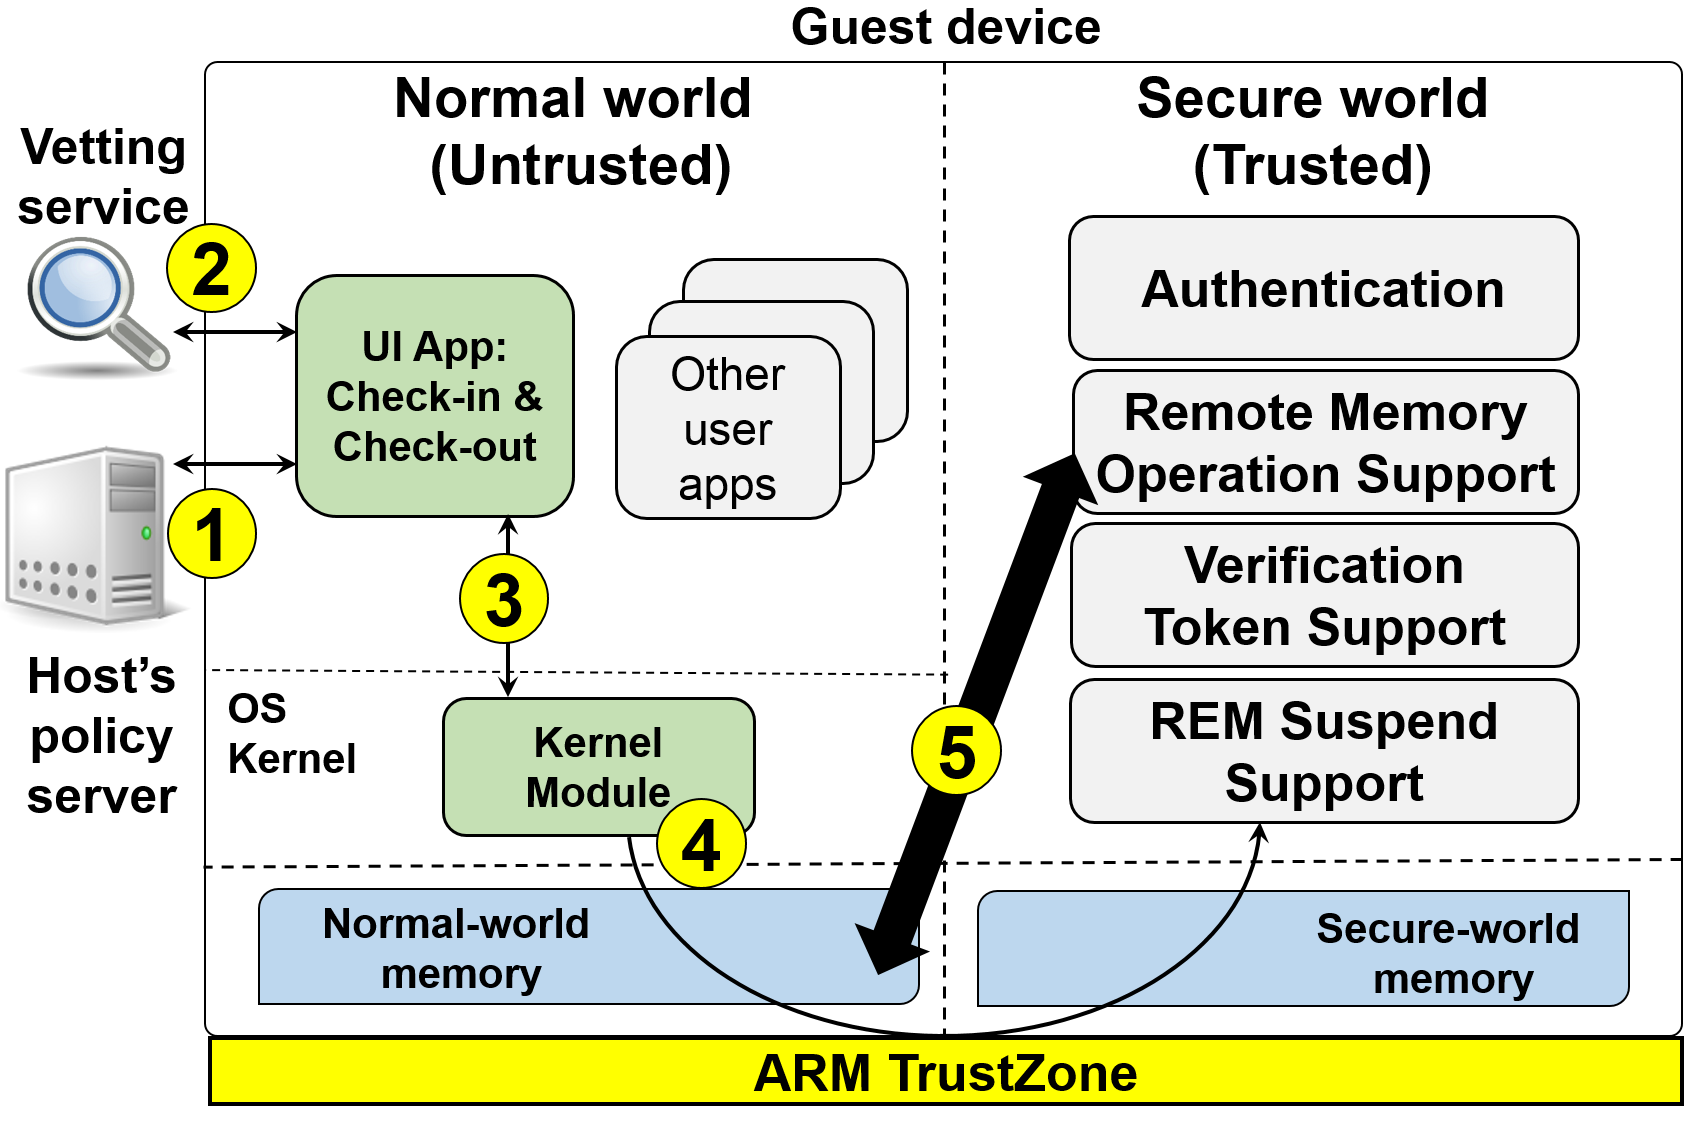
\includegraphics[keepaspectratio=true,width=0.45\textwidth]{figures/overall-design.png}\\
%\indent\vspace{-0.4cm}
\multicolumn{1}{|p{0.47\textwidth}|}
{\small \circone~The host communicates with the UI app on the guest and sends
requests to perform remote memory operations. 
%
\circtwo~The UI app uses the vetting service to determine the safety of the
request. 
%
\circthree~If determined to be safe, the UI app forwards this request to the
supporting kernel module. 
%
\circfour~The kernel module invokes the secure world by performing a world
switch. 
%
\circfive~The secure world performs the requested memory operations on the
normal world memory on behalf of the host.  The components in the normal world
(the UI app and kernel module) are untrusted. We rely on ARM TrustZone's secure
boot to establish trust in the secure world.}\\
\hline
\end{tabular}
\end{center}
\indent\vspace{-0.5cm}
\mycaption{Guest device setup showing components of the policy enforcement
mechanism.}{\label{figure:overall}}
\end{figure}

Guest devices are therefore set up as shown in \figref{figure:overall}.  Within
the normal world, the end-user's interface is a user-level app (called the UI
app) that allows him to interact with the host for device check-in and
check-out. The app interacts with the components in the secure world via a
kernel module. The host sends a request to perform remote memory operations on
the guest device to the app. The app determines the safety of this request
using the vetting service (\sectref{section:vetting}), and forwards the request
to the kernel module, which invokes \textsf{smc} to world switch into secure
world. The components of the secure world then perform the request and
communicate any return values to the host via the UI app. All messages include
a message-authentication code computed using a key established during the
mutual authentication step.

We do not place any restrictions on how the host and guest device communicate.
Thus, the host's policy server could be hosted on the cloud and communicate
with the guest device over WiFi or 3G/4G. Alternatively, the host could install
physical scanners at a kiosk or on the entry-way to the restricted space.  Guest
devices would use Bluetooth, NFC, or USB to pair with the scanner and use it to
communicate with the host.

The core mechanisms that run in the secure world of the guest device have two
key features. They are \textit{policy-agnostic} in that the same mechanisms can
be used to enforce a variety of host policies. The narrow read/write interface
is also \textit{platform-agnostic}, and allows the same mechanisms to work
irrespective of whether the normal world runs Android, iOS or Windows. This
approach shifts complex device analysis and policy formulation tasks to the
hosts. Hosts would naturally need to have separate modules to analyze and
formulate memory updates for various normal world OSes.

\subsection{Authentication}
\label{section:mechanism:auth}
\newcommand{\ks}{$k_s$}
\newcommand{\pub}[1]{{\sf PubKey#1}}
\newcommand{\prv}[1]{{\sf PrivKey#1}}
\newcommand{\enc}[2]{\textsf{Enc}$_{#1}$(#2)}
\newcommand{\cert}[1]{\textsf{Certificate}(#1)}

The host and guest device begin by mutually authenticating each other
(\figref{figure:authentication}). We assume that both the host and the guest
device have public/private key pairs with digital certificates issued by a
certifying authority. The guest device stores its private key \prv{G} in its
secure world, thereby protecting it from the untrusted normal world. 

\begin{figure}[t!]
\footnotesize
\renewcommand{\arraystretch}{0.85}
\centering
\begin{tabular}{|rll|}
\hline
\multicolumn{3}{|l|}{Let host's public/private keypair be \pub{H},~\prv{H}.}\\
\multicolumn{3}{|l|}{Let guest's public/private keypair be \pub{G},~\prv{G}.}\\
1. & \textbf{Guest} $\rightarrow$ \textbf{Host}:
   & \pub{G}, \cert{\pub{G}}\\
%
2. & \textbf{Host} $\rightarrow$ \textbf{Guest}:
   & \pub{H}, \cert{\pub{H}}\\
%
3. & \multicolumn{2}{p{0.42\textwidth}|}{Guest and host verify
       \cert{\pub{H}} and \cert{\pub{G}}}\\
%
4. & \textbf{Host} $\rightarrow$ \textbf{Guest}:
   & $M$, \enc{\prv{H}}{$M$} (\ie~host signs $M$),\\
%
   & \multicolumn{2}{p{0.42\textwidth}|}{where $M$ is 
        \enc{\pub{G}}{\ks, timestamp}}\\
%
5. & \multicolumn{2}{p{0.42\textwidth}|}{Guest verifies host's digital 
        signature, decrypts M to obtain \ks, and checks timestamp}\\
%
\hline
\end{tabular}
\mycaption{Mutual authentication and establishment of \ks.}
{\label{figure:authentication}}
\end{figure}

Authentication is akin to SSL/TLS handshakes. The host and the guest exchange
public keys and validate the certificates of these keys with the issuing
authority. The host then computes a session key \ks, which is then transmitted
to the client over a secure channel. Note that \ks\ is only used to protect
the integrity of messages transmitted between the guest and the host and not
their secrecy. The key \ks\ is stored in secure world memory, and is invisible
to the normal world. It persists across REM-suspends of the guest device, but 
is erased from memory if the device is rebooted.

\addtext{Task 8}{
As with SSL/TLS, the ability of this protocol to resist man-in-the-middle
attacks depends on the host and guest device's ability to validate each other's
public keys. We assume that device vendors would provision \pub{G} for
individual devices and register them with a certifying authority. Hosts
register \pub{H} in much the same manner as is done for Web services today.
While there is a case to be made that the certifying authority model has its
limitations in the era of the Web and smart devices~\cite{sokssl:oak13}, we
note that our use of authentication is entirely standard---to validate the
host's and guest device's identities and to establish a session key \ks.  Thus,
we think that the other parts of our policy enforcement mechanism will work
as-is with alternative authentication schemes, \eg~those that use
identity-based encryption.
}


\subsection{Remote Reads and Writes}
\label{section:mechanism:rmo}

\myparagraph{Remote Reads} 
%
During check-in the host typically requests the guest to send raw memory pages
from the normal world for analysis.  The UI app receives this request and
performs a world switch to complete the request.  The world switch suspends the
UI app and transfers control to the secure world.  Each request is a set (or
range) of virtual memory addresses of pages that must be sent to the host.  The
host also includes a message-authentication code, a SHA1-based HMAC in our
case, with the request. The HMAC is computed on the body of the request using
the key \ks\ negotiated during authentication.

The secure world checks the integrity of the request using the HMAC. This step
is necessary to ensure that the request was not maliciously modified by the
untrusted components in the normal world. The secure world then translates each
virtual page address in the request to a physical page address by consulting
the page table in the normal world kernel. In this case, the page table will
correspond to the suspended context in the normal world, \ie~that of the UI
app, into which the running kernel is also mapped.  It then creates a local
copy of the contents of this physical page from the normal world, and computes
an HMAC over the page (again using \ks). The page and its HMAC are then copied
to a buffer in the normal world, from where they can be transmitted to the host
by the UI app.  The host checks the HMAC and uses the page for analysis. This
process could be iterative, with the host requesting more pages from the guest
device based upon the results of the analysis of the memory pages received up
to that point.

Both the host and the secure world are isolated from the normal world, which is
untrusted. We only rely on the normal world kernel to facilitate communication
between the host and the secure world. Moreover, both the host and the secure
world use HMACs to protect the integrity of messages transmitted via the normal
world.  The normal world may drop messages and cause a denial-of-service
attack; however, such attacks are outside our threat model (see
\sectref{section:threat}). The host can therefore reliably obtain the memory
pages of the normal world to enable the kinds of analyses described in
\sectref{section:policy}. Communication between the host and the secure world
is not confidential and is therefore not encrypted.\footnote{The host and guest
could communicate over SSL/TLS, but this channel on the guest ends at the UI
app, which runs in the normal world.} Thus, a malicious normal world kernel can
potentially snoop on the requests from the host to fetch pages and attempt to
remove the infection to avoid detection. However, this would have the desirable
side-effect of cleaning the guest device at check-in.

\myparagraph{Remote Writes}
%
The host reconfigures the guest by modifying the running state of the normal
world kernel via remote memory updates. The host sends the guest a set of
triples
$\langle$\textit{vaddr}$_i$,~\textit{val}$_i$,~\textit{old-val}$_i$$\rangle$
together with an HMAC of this request. The normal world conveys this message to
the secure world, which verifies its integrity using the HMAC.  For each
virtual address \textit{vaddr}$_i$ (which refers to a memory location in the
virtual address space of the UI app) in the request, the secure world ensures
that the current value at the address matches \textit{old-val}$_i$. If
\textit{all} the \textit{old-val}$_i$ values match, the secure world replaces
their values with \textit{val}$_i$; else the \textit{entire} operation is
aborted.

Because the normal world is frozen during the course of this operation, the
entire update is atomic with respect to the normal world. When a remote write
operation succeeds, the secure world computes and returns a verification token
to the host. If not, it returns an \textsc{Abort} error code denoting failure.

The host's memory update request is aborted if the value stored at
\textit{vaddr}$_i$ does not match \textit{old-val}$_i$.  This design feature is
required because the host's remote read and write operations do not happen as
an atomic unit. The host remotely reads pages copied from the normal world's
memory, analyzes them and creates remote write request using this analysis.
During this time, the normal world kernel continues to execute, and may have
updated the value at the address \textit{vaddr}$_i$.

If the memory update is aborted, the host repeats the operation until it
succeeds. That is, it refetches pages from the guest, analyzes them, and
creates a fresh update. In theory, it is possible that the host's memory
updates will abort \textit{ad infinitum}. However, for the setting that we
consider, aborts are rare in practice. This is because our
write operations modify the addresses of peripheral device driver hooks.
Operating systems typically do not change the values of device driver hooks
after they have been initialized at system boot. 

In theory, a remote memory write can also abort if the virtual address
\textit{vaddr}$_i$ referenced in the request is not mapped to a physical page
in memory, \ie~if the corresponding page has been swapped out to persistent
storage. In practice, however, we restrict remote writes to kernel data pages
that are resident in physical memory, as is the case with device drivers and
pages that store data structures of peripherals. Thus, we do not observe
\textsc{Abort}s due to a failure to resolve \textit{vaddr}$_i$s.

It is possible to completely avoid such problems by designing the both the read
and write operations to complete within a single world switch. During this
time, the normal world remains frozen and cannot change the view of memory
exported to the host. The read and write operations will therefore happen as an
atomic unit from the normal world's perspective. However, in this case, the
secure world must have the ability to directly communicate with the host. As
previously discussed, we decided against this design because it has the
unfortunate consequence of bloating the functionality to be implemented in the
secure world.  Thus, we make the practical design tradeoff of minimizing the
functionality of the secure world while allowing the rare remote write failure
to happen.

\addtext{Task 15}{Note that our approach uses virtual addresses in remote
memory operations. In doing so, we implicitly trust the integrity of page
tables in the normal world kernel, which are used to translate these virtual
addresses to physical ones. Recent work has demonstrated address-translation
redirection (ATRA) attacks that work by maliciously modifying page table
entries and the page table base register~\cite{atra:ccs14}. An ATRA attack
effectively hides malicious code and data modifications by creating shadow
pages containing unmodified code and data, and maliciously modifying page table
entries to redirect requests from a security monitor to these shadow pages.  On
ARM TrustZone devices, it is possible to defend against such attacks by
ensuring that all normal world page table updates are shepherded by the secure
world. This is implemented by modifying the normal world kernel to invoke the
secure world (via \textsf{smc}) for page table updates, and implementing a
suitable security policy within the secure world to ensure the integrity of
these updates~\cite{knox:ccs14,sprobes:most14}. We have not implemented this
defense in our prototype and doing so will require additional code in the
secure world. However, we note that such a defense is already implemented as
part of the secure world in Samsung Knox~\cite{knox:ccs14}. We hypothesize that
a solution that integrates our approach with Knox will therefore be robust
against ATRA attacks.}

\subsection{Verification Tokens}
\label{section:mechanism:tokens}

The host receives a verification token from the secure world upon successful
completion of a remote write operation that updates normal world memory. 
A verification token \textsf{VTok}[$r$] is the following value:
%
%\begin{center}
%
$
r||\textit{MemState}||\textsf{HMAC}_{k_s}[r||\textit{MemState}]$
%
%\end{center}
%
where \textit{MemState} is
$\langle\textit{vaddr}_1,~\textit{val}_1\rangle||\ldots||\langle\textit{vaddr}_n,~\textit{val}_n\rangle$,
the set of \textit{vaddr}$_i$ modified by the remote write, and the new values
\textit{val}$_i$ at these locations. The token \textsf{VTok}[$r$] is
parameterized by a random nonce $r$. This nonce can either be provided by the
host together with the remote write request, or can be generated by the secure
world. 

Verification tokens allow the host to determine whether the guest attempted to
revert the host's memory updates, either maliciously or by turning off the
guest device. To do so, the host obtains a verification token
\textsf{VTok}[$r_{{\it checkin}}$] upon completion of check-in, and stores this
token for validation. During checkout, the host requests a validation token
\textsf{VTok}[$r_{\it checkout}$] from the guest over the same virtual memory
addresses. The secure world accesses each of these memory addresses and
computes the verification token with $r_{\it checkout}$ as the nonce. The host
can compare the verification tokens \textsf{VTok}[$r_{{\it checkin}}$] and
\textsf{VTok}[$r_{{\it checkout}}$] to determine whether there were any changes
to the values stored at these memory addresses. 

The nonces $r_{\it checkin}$ and $r_{\it checkout}$ ensure the freshness of
the tokens
\textsf{VTok}[$r_{{\it checkin}}$] and \textsf{VTok}[$r_{{\it checkout}}$].
The use of \ks\ to compute the HMAC in the verification token ensures that the
token is only valid for a specific device and for the duration of the session,
\ie~until check-out or until the device is powered off, whichever comes
earlier. Because \ks\ is only stored in secure world memory, it is ephemeral
and unreadable to the normal world. Any attempts to undo the host's memory
updates performed at check-in will thus be detected by the host.

% \subsection{Security Analysis}
% What if kernel module is loaded dynamically? We disable that.

\subsection{Restricted Space Mode (REM) Suspend}
\label{section:mechanism:REMsuspend}

\newcommand{\kdev}{{\sf K$_{\sf Dev}$}}
%
If a guest device is rebooted, the host's updates to device memory are undone
and \ks\ is erased from secure world memory, thereby ending the session.
However, it is sometimes necessary to suspend the device in the restricted
space, \eg~to conserve battery power. We design REM-suspend to handle such
cases and allow the session key \ks\ to persist when the device is woken.

The ARM TrustZone allows a device to be configured to route certain interrupts
to the secure world~\cite{armtz}. We route and handle power-button presses and
low-battery events in the secure world by prompting the user to specify whether
to REM-suspend the device. When a guest device is checked into a restricted
space, we configure the default power-down option to be REM-suspend; the
default reverts to the traditional power-down sequence when the device checks
out. The user can consciously choose to bypass REM-suspend, in which case the
device shuts down the traditional way, thus ending the session. The same
happens if the device shuts down due to other causes, \eg~power loss caused by
removing the device's battery. 

When the guest device REM-suspends, the secure world checkpoints normal world
memory, which contains the host's updates, and the key \ks, which are both
restored when the device is woken up. The main challenge is to protect the
confidentiality of \ks. The device user is untrusted, and can read the contents
of persistent storage on the device; \ks\ must thus be stored encrypted with a
key that is not available to the device user.

To achieve this goal, we leverage a feature referenced in the ARM TrustZone
manual~\cite[\S6.3.1]{armtz}, which provisions a device with a
statistically-unique one-time programmable secret key that we will refer to as
\kdev. \kdev\ is located in an on-SoC cryptographic accelerator, and accessible
only to secure world software~\cite[\S6.3.1]{armtz}. \kdev\ cannot be read or
changed outside the secure world, other bus masters or the JTAG~\cite{jtag}.
\kdev\ allows confidential data to be encrypted and bound to the device, and
has previously been referenced in other
research~\cite{tlr:asplos14,sentry:asplos15,ftpm:msrtr,mobiletrustedcomputing:ieee14}.
Note that \kdev\ is not the same as \prv{G}, the device's private key.

In REM-suspend, the secure world first checkpoints normal world memory and CPU
registers, and suspends the execution of the normal world. It sets a bit
\textsf{B$_{\sf REM}$} to record that the device is REM-suspended. It stores
the checkpoint and \textsf{B$_{\sf REM}$}, together with an HMAC of these
values under \ks\ on the device's persistent storage. It also stores to
persistent storage the value of \ks\ encrypted under \kdev.  The untrusted
device user does not know \kdev, and therefore cannot forge the encrypted value
of \ks\ or retrieve the cleartext value of \ks. The HMACs under \ks\ protect
the integrity of the normal world checkpoint and \textsf{B$_{\sf REM}$}.
\addtext{Task 6}{An alternative way to protect the integrity of the normal
world checkpoint and \textsf{B$_{\sf REM}$} is to store them in the
replay-protected memory block (RPMB), a trusted storage partition available on
many mobile devices that come equipped with a embedded multi-media storage
controller. The RPMB offers integrity-protection for stored data, ensures data
freshness by protecting against replay attacks, and has been leveraged in
recent work~\cite{ftpm:msrtr}. However, even with this alternative the
confidentiality of \ks\ needs to be protected by encrypting it using \kdev.}

When the device is woken up, the secure world uses \textsf{B$_{\sf REM}$} to
check if the device is REM-suspended. If so, it uses \kdev\ to retrieve \ks,
verifies the integrity of the normal world checkpoint and \textsf{B$_{\sf
REM}$} using their HMACs, and starts the normal world from this checkpoint.
The device resumes execution under the same session and continues to
produce verification tokens if requested by the host.

\addtext{Task 6}{The original ARM TrustZone manual~\cite{armtz} described
\kdev\ in the context of a hypothetical device, and \kdev\ is not part of the
core specification of the TrustZone architecture. As such, it is not clear how
many deployed devices support \kdev; for example, it is not supported by the
TrustZone-enabled board that we used for our prototype implementation.  Many
emerging ARM TrustZone-based security
solutions~\cite{tlr:asplos14,sentry:asplos15,ftpm:msrtr} rely on the existence
of \kdev, and it is likely that future revisions of the TrustZone architecture
will incorporate such a key. The REM-suspend protocol can be used on any
device that supports \kdev\ or a cryptographic key with similar properties,
\ie~a hardware-provisioned key only accessible from the secure world. 
Note that guest devices that do not support such a key can still be
restricted using our approach. However, the only shortcoming is that without
REM-suspend, a power-down event will undo the memory updates requested by the
host, and clear \ks, thereby terminating the session with the host.}
